\title[JASA/draft]{Under-ice acoustic navigation using real-time model-aided range estimation}
\author{EeShan C. Bhatt}
\email{ebhatt@whoi.edu}
\affiliation{MIT-WHOI Joint Program in Oceanography/Applied Ocean Science \& Engineering, Cambridge and Woods Hole, MA, USA}
\affiliation{Department of Mechanical Engineering, Massachusetts Institute of Technology, Cambridge, MA}
\author{Oscar Viquez}
\affiliation{Department of Mechanical Engineering, Massachusetts Institute of Technology, Cambridge, MA}
\author{Henrik Schmidt}
\email{henrik@mit.edu}
\affiliation{Department of Mechanical Engineering, Massachusetts Institute of Technology, Cambridge, MA}

% \author{Author Four}
% \email{author.four@university.edu}
% \affiliation{Department2,  University2, City, State ZipCode, Country}

\preprint{Bhatt, JASA}   %  if you want want this message to appear in upper right corner of title page

\date{\today}

% The motivation behind this work is to improve the standard LBL navigation’s conversion of travel time to range for an under-ice environment in a way that could be generalized to any acoustic waveguide. To do this, we introduce the Minimal Bounce Criteria method to operationalize real-time acoustic modeling into an effective horizontal group velocity estimate.

% 	This system was implemented on an autonomous underwater vehicle (AUV) on multiple missions, including an 11 km untethered, under-ice deployment, in March 2020. The AUV was deployed through a hydrohole from Topside and due to a disk error, stalled underneath the ice surface while transmitting its perceived location. The AUV was found within a meter away from its reported location, which serves as strong (but qualitative) evidence of the navigation performance provided by the single group velocity calculation. Because the navigation updates throughout the AUV mission have no GPS ground truth to compare to, this paper evaluates the same system performance across the GPS-navigated LBL beacons. 

% 	The real-time error from the Nearest Bounce Criteria (NBC) achieves a mean absolute positioning error of 11 m. Upon further evaluation of the acoustic events, the Minimal Bounce Criteria (MBC) is run in the same automated pipeline in post-processing (akin to real-time computational constraints and needs) and achieves an error of roughly 3 m.

% 	Both the NBC and MBC pseudorange estimations are compared to the GPS data on the LBL beacons. The error itself is small and the pattern of error exhibited indicates that the GPS ground truth data has significant noise (drift) that is not replicated by either pseudorange estimation method. For the MBC in particular, the post-processing error is within the precision of the GPS sensor, suggesting that its performance rivals that of GPS.

\begin{abstract}
The long baseline (LBL) underwater navigation paradigm relies on the conversion of recorded travel time to range to trilaterate for position.
For real-time operations, this conversion assumes an isovelocity sound speed.
For re-navigation in post-processing, computationally and/or labor intensive acoustic modeling may be employed to reduce uncertainty driven by multipath arrivals.
This work demonstrates a real-time ray-based prediction method of the effective horizontal group speed to minimize vehicle position error.
\llabel{2.1} This method was implemented for a small scale AUV-LBL system in March 2020, in the Beaufort Sea, in total under-ice conditions and a double ducted acoustic propagation environment.
The vehicle was successfully deployed and recovered.
\llabel{2.2} Given the lack of GPS data throughout the vehicle's mission, however, the localization performance between GPS-linked beacon-to-beacon connections serves as a proxy for the effectiveness of this approach.
The real-time positioning error between beacons was roughly 11 meters at distances up to 3 km, matching the magnitude of corrections recorded by the AUV during field operations.
In post-processing, the localization performance is reevaluated with an operationally equivalent navigation stack using modeled, historical, and locally observed sound speed profiles for a Minimal Bounce Criteria (MBC), as deployed in real-time, and an improved ray filtering algorithm, the Nearest Bounce Criteria (NBC).
The best performing median re-positioning errors by bounce criterias are roughly 10 and 2 meters, respectively.
\llabel{2.3} Further investigation suggests that the GNSS ground truth data have some noise that is not reciprocated in the travel time data.
Re-trilateration suggests that this approach effectively extends the single meter accuracy of the deployed GNSS pucks into the water column.
\end{abstract}

%% pacs numbers not used

\maketitle

% =========================================================================== %
% =========================================================================== %

\section{Introduction}
\label{sec:1}  
Autonomous underwater vehicles (AUVs) are increasingly capable platforms to explore and sample the ocean, particularly for remote and/or dangerous regions.
However, navigation uncertainty is a major challenge in considering AUVs as standard tools for oceanographic research.
While land and air-based robots utilize information from Global Navigation Satellite Systems (GNSS) to achieve stunning location accuracy and precision throughout the duration of their missions, AUVs cannot access GNSS while underwater due to the rapid attenuation of electromagnetic waves.
Therefore, underwater vehicles have relied on any combination of dead reckoning, hydrodynamic models, inertial navigation systems, doppler velocity logs, and acoustic baseline positioning systems for navigation \citep{paull_auv_2014}.
Limiting navigation error and drift requires an AUV to periodically stall on the surface and obtain a GNSS fix to reset its position error.
This foolproof method of self-positioning is undesirable for stealth, adverse weather conditions, and mission efficiency, and inaccessible in a GPS-denied situation like an ice-covered environment.

% introduce LBL and precise statement of work
Of acoustic baseline navigation systems, long baseline (LBL) is the most GPS-like in style and scale, and most appropriate for mitigating drift without overburdening computation or payload size on the vehicle \citep{paull_auv_2014,van_uffelen_global_2021}.
The state-of-the-art for LBL outsources depth to a pressure sensor and solves the two-dimensional localization problem by assuming an isovelocity, linear scaling between one way travel time (OWTT) and range \citep{eustice_recent_2006,eustice_experimental_2007,webster_preliminary_2009,webster_advances_2012}.
This assumption is valid for short scale operations but oversimplifies propagation for larger and/or complex acoustic environments.
This paper demonstrates an embedded model-aided data processing approach to convert recorded OWTTs into pseudorange estimates.
This approach was necessitated by total under-ice conditions and a double ducted acoustic environment, in the Beaufort Sea, in March 2020, for an AUV deployment during the Ice Exercise 2020 (ICEX20).
We quantify the success of the proposed acoustic ranging method using GPS-linked beacon-to-beacon communication events, as the AUV-LBL positioning has no ground truth GNSS to compare to.

%% rest of the background, JASA style

% PNT
For clarity, we introduce definitions for timing, positioning, and navigation. 

% More about LBL navigation
While RAFOS floats have championed one way ranging for re-positioning \citep{rossby_rafos_1986,duda_evaluation_2006}, the ability to do so for navigation was facilitated by \llabel{1.11} the advent of the WHOI micro-modem \citep{singh_underwater_2006} and synchronized chip scale atomic clocks \citep{gardner_second_2016}.
Several short range (less than ten kilometers) navigation efforts have achieved minimal error with a nominal sound speed value \citep{eustice_experimental_2007,webster_preliminary_2009,kepper_mems_2017}.
However, these efforts were all conducted with X sound speed conditions.
The approach in this paper, and other related works, was specifically designed to... the recently observed double ducted sound speed profile...
For convenience, we call this phenomena the Beaufort Lens, with the lens referring to ... 

There is no comparable work in the Arctic for a short scale AUV deployment in the Beaufort Lens. 
Both seminal and more recent AUV deployments witnessed the classical upward refracting sound speed profile that is amenable to an isovelocity simplification.
Of note are large scale glider deployments; these, however, operated at X depths, X spatial scales, and did not need precise navigation because they experienced little to no sea ice.
At larger scales on the order of hundreds of kilometers, a deterministic \citep{graupe_preliminary_2019} or through-the-sensor \citep{webster_towards_2015} value for sound speed was used, but error remained in the hundreds of meters.
The sound speed value was chosen by...

The navigation approach proposed includes a non-deterministic relationship between travel time and range previously limited to large scale re-navigation and re-positioning efforts.
Such post-processing efforts can utilize additional information or computation that is inaccessible for onboard computation.

\begin{figure}[h!]
	\centering
	\includegraphics[width=\columnwidth]{figs/auv-track-update.png}
	\caption{The under-ice mission track for AUV Macrura, including the position updates as it stalled underneath the ice overnight. A marker was placed on the ice at the vehicle's estimated self-location. It was recovered after a three day storm within a meter of the marker.}
	\label{fig:vehicleRecovery}
\end{figure}
% include story later on and cite this figure?

\clearpage
\section{ICEX20 conditions and experiment design}

\begin{figure}[h!]
	\centering
	\includegraphics[width=\reprintcolumnwidth]{figs/ssp-gvel-icex20-icex16.pdf}
	\caption{Anticipated sound speed conditions: finish this using stuff from ICEX16, HYCOM, ITP}
	\label{fig:sspExpectation}
\end{figure}

\begin{figure}[h!]
	\centering
	\includegraphics[width=\textwidth]{figs/Fig2.pdf}
	\caption{A schematic overview of the Integrated Communication and Navigation Network (ICNN), which provides joint data-transfer and tracking between AUV and a human decision maker at Topside.}
	\label{fig:icnnOverview}
\end{figure}

\begin{figure}[h!]
  \centering
  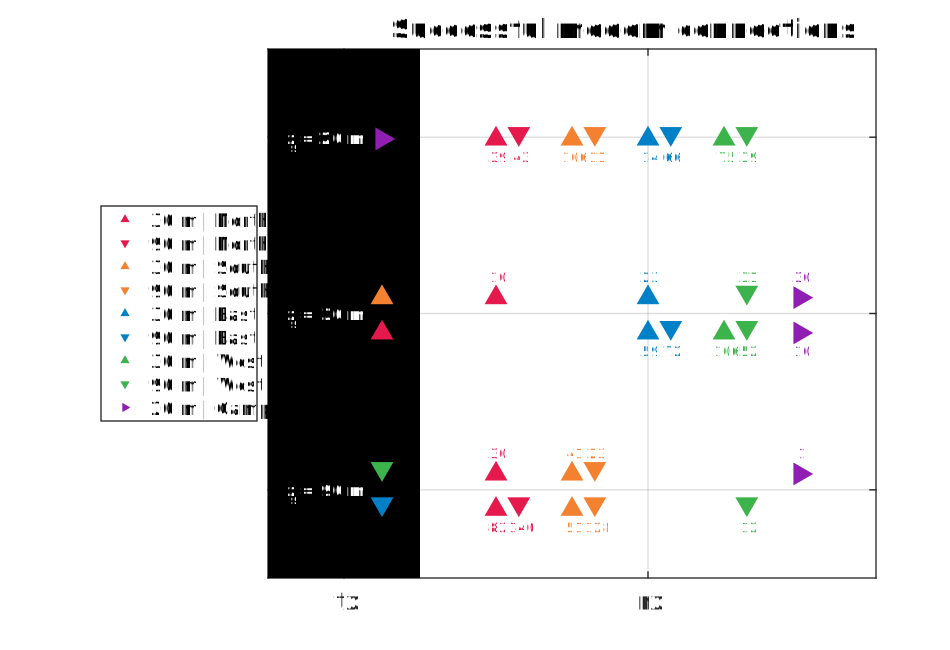
\includegraphics[width=\textwidth]{figs/modem-chart.pdf}
  \caption{An overview of the modem experiment by source and receiver depth and position. The black column on the left, $tx$, shows the source depth, $z_s$. The column on the right, $rx$, shows the receivers with the amount of good contacts. The orientation of the triangles\textemdash sideways, upwards, and downwards\textemdash corresponds to depths of 20, 30, and 90 m.}
  \label{fig:overview}
  \end{figure}

\clearpage
\section{\label{sec:realtime} Real-time pseudorange analysis}

\subsection{Minimal bounce criteria (MBC)}

\subsection{Pseudorange error metrics}

\subsection{Inherent overestimation from the minimal bounce criteria}

\subsubsection{Source depth of 20 m}
\begin{figure}[h!]
  \centering
  \includegraphics[width=\reprintcolumnwidth]{figs/Fig4.pdf}
  \caption{Eigenrays for beacon to beacon events for each sound speed with a nominal source depth of 30 m. The beacons are highlighted in color/marker coding in Fig. \ref{fig:overview}. The eigenrays are curated from BELLHOP by travel time proximity and are traced in the representative receiver colors over a total ray fan in gray.}
  \label{fig:raytrace-zs20}
\end{figure}


\subsubsection{Source depth of 30 m}
\begin{figure}[h!]
  \centering
  \includegraphics[width=\reprintcolumnwidth]{figs/Fig4.pdf}
  \caption{Eigenrays for beacon to beacon events for each sound speed with a nominal source depth of 30 m. The beacons are highlighted in color/marker coding in Fig. \ref{fig:overview}. The eigenrays are curated from BELLHOP by travel time proximity and are traced in the representative receiver colors over a total ray fan in gray.}
  \label{fig:raytrace-zs30}
\end{figure}

\subsubsection{Source depth of 90 m}
\begin{figure}[h!]
  \centering
  \includegraphics[width=\reprintcolumnwidth]{figs/Fig4.pdf}
  \caption{Eigenrays for beacon to beacon events for each sound speed with a nominal source depth of 30 m. The beacons are highlighted in color/marker coding in Fig. \ref{fig:overview}. The eigenrays are curated from BELLHOP by travel time proximity and are traced in the representative receiver colors over a total ray fan in gray.}
  \label{fig:raytrace-zs90}
\end{figure}

\clearpage
\section{\label{sec:post} Post-processed pseudorange analysis}

\subsection{Nearest bounce criteria (NBC)}

\subsection{Effective sound speed predictions}

\begin{figure}[h!]
\includegraphics[width=\columnwidth]{figs/Fig5.pdf}
\caption{A comparison of group velocity predictions for all beacon to beacon events in post-processing with a source depth of 30 m, with group velocity on the y-axis and recorded travel time on the x-axis. The left panel is for a receiver depth of 30 m; the right panel for 90 m. The sound speed source is indicated by color. The minimal and nearest bounce criterion are distinguished by different marker shapes, compared to the separately colored red dots showing the naive, data-driven group velocity calculation.}
\label{fig:gvel30}
\end{figure}

\subsection{Pseudorange error metrics}

\begin{figure}[!ht]
\includegraphics[width=\textwidth]{figs/Fig6.pdf}
\caption{The post-processed range error for source depths of 20, 30, and 90 m, and receiver depths of 30 and 90 m. The dashed gray line shows no error. The shaded region connects the range performance across all events.}
\label{fig:rangeError}
\end{figure}

\section{Re-positioning using the nearest bounce criteria}

\begin{figure}[h!]
\includegraphics[width=\textwidth]{figs/Fig7.pdf}
\caption{\label{fig:compareV1V2}{A comparison of range estimation error for all beacon to beacon events in post-processing. From left to right, the SSPs are the baseline, the chosen weights, and HYCOM. The colors indicate the source depth, darkening with depth, and the shapes indicate the multipath structure. Because this plot is square, the shaded region shows where the updated algorithm is less accurate than the \textit{in situ} algorithm.}}
\end{figure}

\begin{figure}[!ht]
\includegraphics[width=\textwidth]{figs/trilat-stat.pdf}
\caption{WRITE THIS.}
\label{fig:trilat}
\end{figure}

\clearpage
\section{Re-navigating AUV data}

FIG A -- error for MBC/NBC (Oscar Fig 6.17). Think about whether to include separate in situ column. Explain why this section uses error whereas previous section uses correction.

I think if we go down this route, we can take out the GNSS noise section entirely. The POMA paper would go over GNSS noise at high latitudes, crossmap, and look at individual drifts. I do not think the crossmap needs to stay in this publication; given small numerical value of the re-positioning trilateration, I think the same point is made (in a better way, actually).

\clearpage
\section{Investigating potential GNSS noise}

\begin{figure}[h!]
	\centering
	\includegraphics[width=\reprintcolumnwidth]{figs/Fig8.pdf} 
	\caption{A comparison of GPS drift (y-axis) versus OWTT drift (x-axis), colored by source and receiver depth. The physical link between North and East are shown on the top; South and West is on the bottom.}
	\label{fig:gps-drift-example}
\end{figure}

\clearpage
\section*{Supplementary Figures}

\subsection*{Ice movement during the modem experiment}
\begin{figure}[h!]
\includegraphics[width=\textwidth]{figs/Fig9.pdf}
\caption{\label{fig:iceFloeDrift}{The ICNN accounts for ice drift throughout the mission duration. This is the magnitude of the ice drift recorded, at each buoy, throughout the modem experiment. The shaded regions reference which sound speed estimate was used.}}
\end{figure}

% ================================================== %
% \begin{figure}[ht]
% \includegraphics[width=\reprintcolumnwidth]{figsamp.jpg}
% \caption{\label{fig:FIG1}{Caption here.}}

% \raggedright
% {\color{red}
% Note: The only figure formats allowed are the following:
% .pdf, .ps, .eps, or .jpg. Figure files must be named in this fashion:
% Figure\#.xxx, where ``\#'' is the figure number and ``xxx'' is the file format
% (Figure1.eps, Figure2.jpg, Figure3a.ps, Figure3b.ps, etc).
% }

% [For these sample pages we have used only figsamp.jpg for convenience]
% \end{figure}
% ================================================== %
\FloatBarrier
\clearpage
\begin{acknowledgments}
We acknowledge the significant operational effort spearheaded by the LAMSS ICEX20 team and all our collaborators.
Bhatt was funded by a National Defense, Science, and Engineering Graduate Fellowship.
This work was supported by the Office of Naval Research 322-OA under ICEX20 (N00014-17-1-2474) and Task Force Ocean (N00014-19-1-2716).

\end{acknowledgments}

\bibliography{sampbib}
